\documentclass{amsart}

\usepackage{graphicx}
\usepackage{caption}
\usepackage{subcaption}

\newtheorem{theorem}{Theorem}[section]
\newtheorem{lemma}[theorem]{Lemma}

\theoremstyle{definition}
\newtheorem{definition}[theorem]{Definition}
\newtheorem{example}[theorem]{Example}
\newtheorem{xca}[theorem]{Exercise}

\theoremstyle{remark}
\newtheorem{remark}[theorem]{Remark}

\numberwithin{equation}{section}

%    Absolute value notation
\newcommand{\abs}[1]{\lvert#1\rvert}

%    Blank box placeholder for figures (to avoid requiring any
%    particular graphics capabilities for printing this document).
\newcommand{\blankbox}[2]{%
  \parbox{\columnwidth}{\centering
%    Set fboxsep to 0 so that the actual size of the box will match the
%    given measurements more closely.
    \setlength{\fboxsep}{0pt}%
    \fbox{\raisebox{0pt}[#2]{\hspace{#1}}}%
  }%
}

\begin{document}

\title{A Proposed Neural Network Activation Function}

\author{Matthew Schroeder}

\date{March 11, 2019}

\begin{abstract}
In this paper a new activation function for deep neural networks is presented.  Their are two variants of the activation function. The first is a smooth, oscillatory version of ReLU. The second is a smooth, oscillatory version of ReLU with exponential decay of the oscillations.
\end{abstract}

\maketitle

\section{INTRODUCTION}
The primary reason neural networks are so successful at solving problems in machine learning is their ability to create highly non-linear functions.   The feature of a neural network which makes this possible is the activation function.  The activation function takes what is otherwise a linear object and makes it non-linear.  It is no surprise then, that discovering new activation functions to use in neural networks is an ongoing area of research.   

The most popular activation function used today is the rectified linear unit (ReLU).  The most attractive property of ReLU seems to be its simplicity; the computation of this function and its derivative is very fast, which simplifies and accelerates the training of neural networks. ReLU, however, is not differentiable at the origin, which has lead to the search for other activation function which are differentiable at the origin and have similar properties.  The purpose of this paper is to present two such activation functions.    

The function which is the basis for the activation functions I will discuss is $$f(x) = \min(1, \max(0, x - \frac{1}{2\pi}\sin(2\pi x)))$$ In the past I have used this function to ramp a servo hydraulic actuator between points. It was chosen since it has continuous first and second derivatives and discontinuities in velocity or acceleration can damage some kinds of specimens (discontinuity in the jerk is tolerated).  A glance at the graph (fig. 1) reveals that this is a Sigmoid function and so, naturally, activation functions came to mind.   

\begin{figure}[tb]
%\blankbox{.75\columnwidth}{3pc}
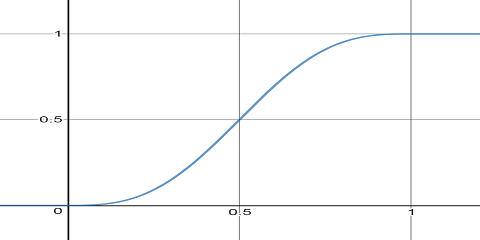
\includegraphics[1]{xsinx.png}
\caption{The graph of f(x) = \min(1, \max(0, x - \frac{1}{2\pi}\sin(2\pi x)))$}
\label{Figure 1}
\end{figure}  

The goal of this paper is not to look at $x-\sin(x)$ as a replacement for the logistic function, but instead is to use $x-\sin(x)$ to create smooth versions of ReLU.   The two activation functions I will consider are shown in the Table 1 (simplest form).  The first is called Oscillating ReLU (OscReLU) )and the second Oscillating ReLU with Exponential Decay (DOscReLU). Both resolve the issue of non-differentiability at zero. 

\begin{table}[!h]
\renewcommand\arraystretch{1.5}
\noindent\[
\begin{array}{|c|c|}
\hline
OscReLU & \max(0, x - \frac{1}{2\pi}\sin(2\pi x)\\
\hline
DOscReLU & \max(0, x - \frac{1}{2\pi}e^{-sx^2}\sin(2\pi x)\\
\hline
\end{array}
\]
\end{table}

This paper is organized as follows. In section 2 ReLU will be discussed. In section 3 the new activation functions are discussed. Section 4 contains an analysis of experimental results.  Finally a conclusion is given in section 5.  

\section{ReLU}  

ReLU was introduced as a replacement for the logistic function and tanh. The formulas for ReLU and its derivative are given by $$f(x) = max(0, x)$$ $$f'(x) = \begin{cases}0 : x < 0 \\ 1 : x \geq 0 \end{cases}$$ The graph of ReLU and of its derivative are shown in Figure 2.  

\begin{figure}[!h]
%\blankbox{.75\columnwidth}{3pc}
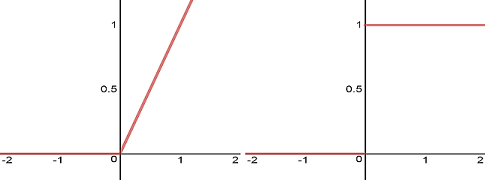
\includegraphics[1]{ReLU.png}
\caption{ReLU and its derivative}
\label{Figure 2}
\end{figure}  

The Logistic function and tanh both have bounded range and have derivatives which asymptotically approach zero (very quickly).  This leads to a phenomena known as the Vanishing Gradient Problem.  Essentially as the gradient goes to zero at a given neuron, it will now longer contribute during back propagation. ReLU solves this problem, at least for positive inputs.  

ReLU is very simple, its use in the network, involves just a comparison, addition and multiplication.  In addition the derivative of ReLU is just a step function. These properties are to be compared with the rather complex formulas and derivative for other activation functions.  The computational simplicity and efficiency of ReLU, coupled with the fact that it works are the reasons it is so popular.   

In addition to ReLU, I will be comparing the performance of OscReLU and DOscReLU to two recent state of the art activation functions: Swish \cite{A} and LiSHT \cite{B}.  
The formulas are given by $Swish(x) = x\dotsigmoid(βx)$ and $LiSHT(x) = x \dot tanh(x)$


\section{OscReLU and DOscReLU}  

The goal of these two activation functions is to introduce a higher level of non-linearity than ReLU, while attempting to maintain many of the favorable properties. The most general formulas for OscReLU and DOscReLU includes parameters. 

\subsection{OscReLU}

OscReLU is a very simple function: 

$$f(x,S,I) = \max(0, (x + S) - \frac{1}{2\pi}\sin(2\pi (x+S)) - I$$  
$f'(x,S,I) = \begin{cases} 1 - cos(2\pi (x+S)) & x \geq -S \\ 0 & x < -S  \end{cases}$$


In Figure 3 is a plot of OscReLU and ReLU.  




\subsection{DOscReLU}  

$DOscReLU(x,S,I,K) = \max(0, (x + S) - \frac{1}{2\pi}e^{-K(x+S)^2}\sin(2\pi (x+S)) - I$
Here S is a horizontal shift which allows the dying gradient of the function to be shifted into the negative half plane, I is a vertical shift, called the inhibitory offset (to be explained below), and, finally, K is the decay rate of the exponential.  


\bibliographystyle{amsplain}
\begin{thebibliography}{10}

\bibitem {A} S.K. Roy, S. Manna, S.R. Dubey, B. Chaudhuri, \textit{LiSHT: Non-Parametric Linearly Scaled Hyperbolic Tangent Activation Function for Neural Networks} ArXIV:1901.05894v1 (2019)

\bibitem {B} P. Ramachandran, B. Zoph, Q.V. Le, \textit{SEARCHING FOR ACTIVATION FUNCTIONS}, ArXIV:1710.05894v1 (2019)

\end{thebibliography}

\end{document}

%------------------------------------------------------------------------------
% End of journal.tex
%------------------------------------------------------------------------------
